\subsection{Data description}
We have a two-class classification problem. The training data $Xtrain$ contains 1500 observations, each 32 dimensional. One training sample has 31 real valued features and 1 categorical feature, the 14th feature. Our task is to predict the category for unseen test data, consisting in 1500 samples. We measure the accuracy of our estimation using RMSE, $0-1 loss$ and $log-loss$. 

\subsection{Data visualization and cleaning}
We noticed the samples were not equally distributed among classes, about $35\%$ of the samples were coming from one class and $65\%$ from the other. We did not have time to study the implications of this on our model estimation. We changed the labelling from -1/1 to 0/1 because our cost function was better expressed using 0 and 1.

The training data were again not centered as seen in $Fig.$ \ref{fig:dist_classification}
After changing feature 14 to a dummy variable we normalized the data to have 0 mean and standard deviation 1. We noticed more outliers in the data of classification than in the one from regression. We removed outliers in a similar way as in the regression task which left us with 1424 samples (5$\%$ of the data were removed).

\begin{figure}[h]
	\begin{subfigure}[b]{0.5\textwidth}
   \includegraphics[width=\textwidth]{figures/classification_distribution.pdf}
    \captionof{figure}{Mean and standard deviation for the training data features. The input is not normalised and contains outliers.}
    \label{fig:dist_classification}
  \end{subfigure}
  \hfill
  \begin{subfigure}[b]{0.45\textwidth}
   \includegraphics[clip, trim=4cm 9cm 3cm 10cm, width=\textwidth]{figures/Lambda_pLG.pdf}
    \captionof{figure}{Train and test error assessment with penalty factor ($\lambda$) for penalized logistic regression for 50-50 split.}
    \label{fig:Lambda_pLr}
  \end{subfigure}
  \hfill
\end{figure}

\subsection{Logistic Regression}

We applied Logistic Regression (logRegression) and Penalized Logistic Regression (penLogRegression) using gradient descent with learning rate $\alpha$.  We obtained the optimal $\alpha$ for logRegression and penalty factor $\lambda$ for penLogisticRegression using the cross validation technique with a $50\%-50\%$ split for training and validation data.

In penLogRegression, the choice of penalty factor $\lambda$ is crucial. We sampled 400 values for $\lambda$s in the interval  $10^{-2}$ to $10^3$. As can be seen in $Fig.$ \ref{fig:Lambda_pLr}, for small $\lambda$ values, training error is much lower than the test error while for large $\lambda$ values the test error gets as high as the training error which is a sign of under-fitting. 
For small $\lambda$ values, the training and test error estimated in penLogisticRegression show very similar behavior with the ones for logRegression. 

The same $\alpha$ value that is obtained for logRegression gives also the best accuracy for penLogisticRegression. Increasing the value of $\alpha$ decreases all error estimations until around $\alpha=0.8$ value which gives the best prediction accuracy for our data.

$Fig.$ \ref{fig:comp_LR_pLR} shows the classification accuracy percentage of logRegression and penLogRegression on the test data using 5-fold cross validation. The improvements with penLogRegression is little but might perform better on unseen data since it is more robust to outliers. Our best accuracy on the test data of $96.348\%$  is obtained using penLogRegression with $\lambda=0.03$ and $\alpha=0.8$. 

For our best setups, we report three types of errors using RMSE, $0-1 loss$ and $log-loss$  in table \ref{table:test_errors}. penLogisticRegression consistently performs better.

\begin{minipage}{\textwidth}
  \begin{minipage}[b]{0.49\textwidth}
    \centering
    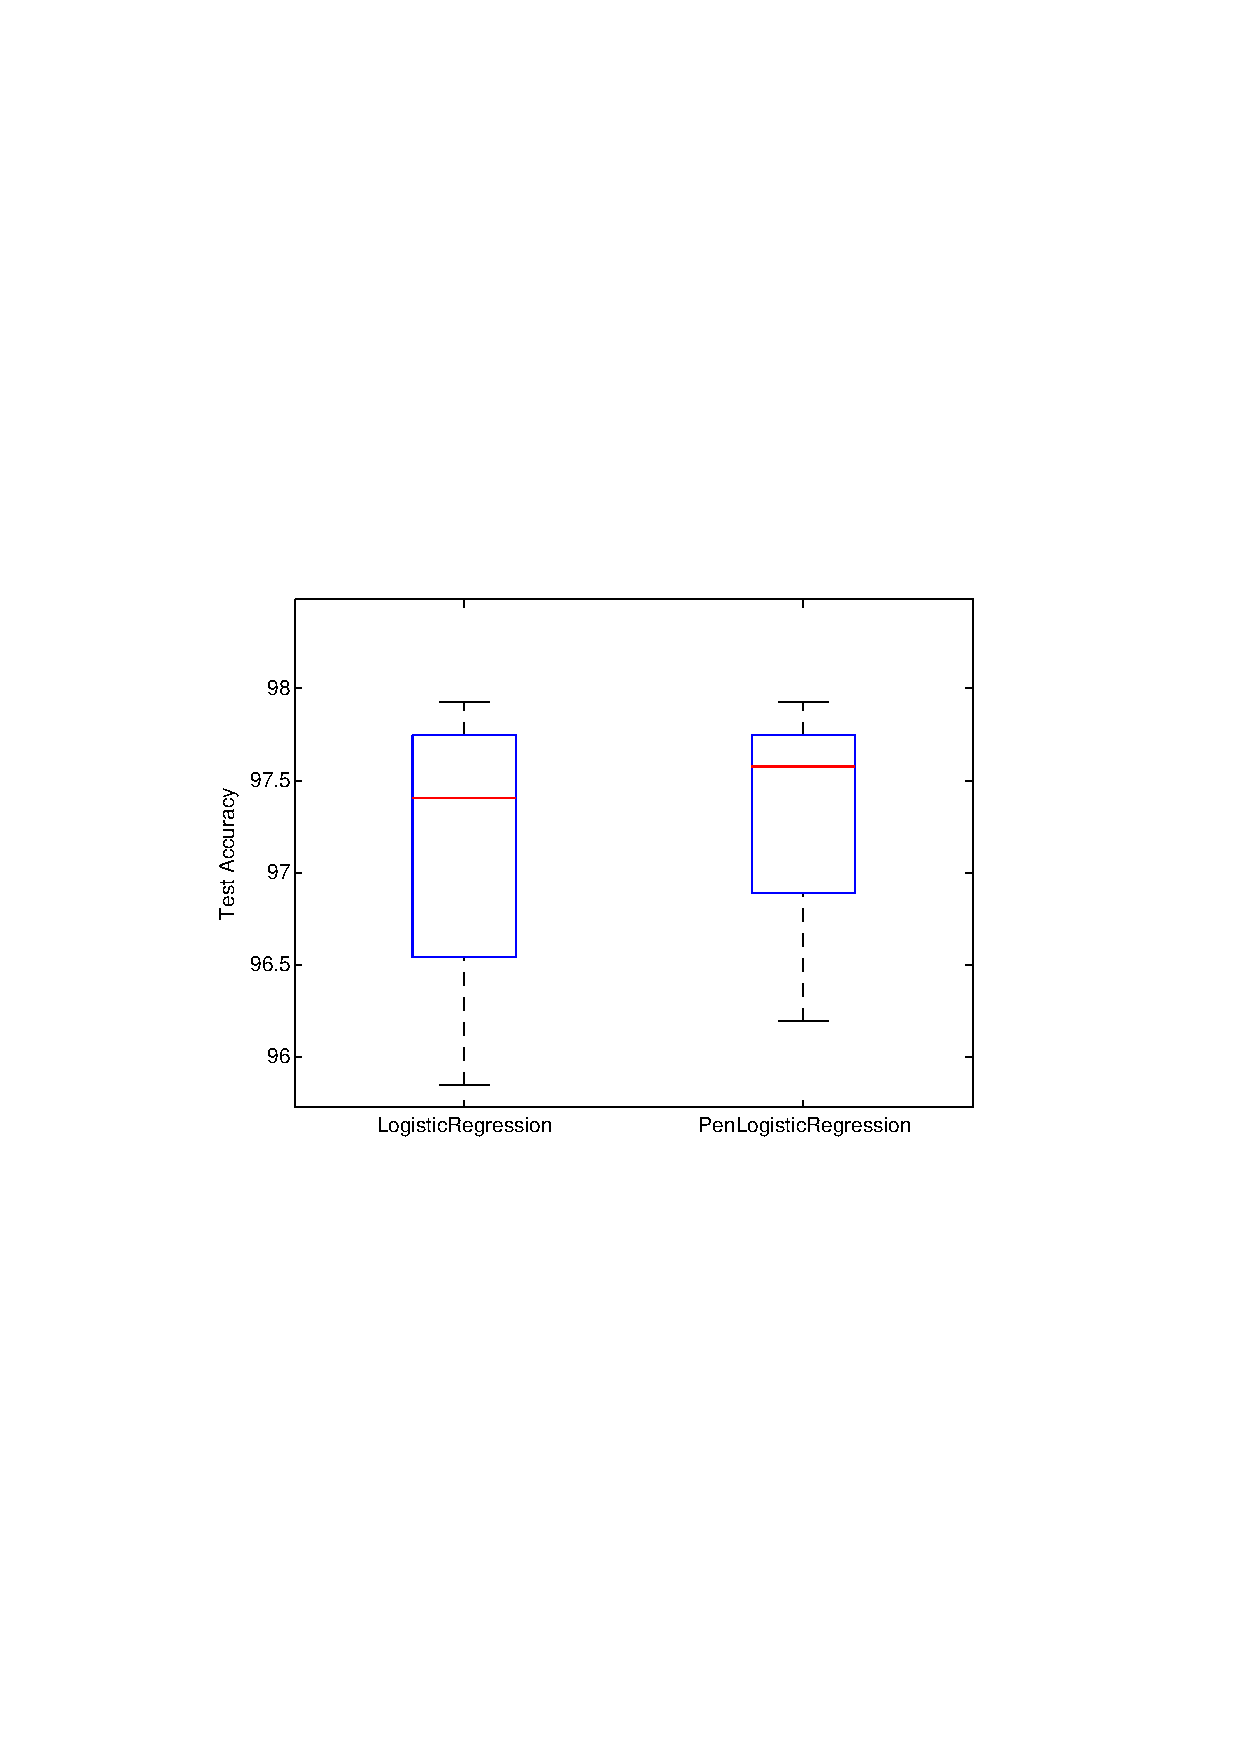
\includegraphics[clip, trim=4cm 10cm 3.5cm 10cm, width=\textwidth]{figures/comparison_LR_pLR.pdf}
    \captionof{figure}{Comparison of logistic regression and penalized logistic regression based on validation accuracy.}
    \label{fig:comp_LR_pLR}
  \end{minipage}
  \hfill
  \begin{minipage}[b]{0.49\textwidth}
    \centering
        \begin{tabular}{ | l | l | l | p{1.2cm} |}
    \hline
    Method & RMSE & 0-1-Loss & Log-Loss \\ \hline
    LogRegression & 0.17 & 0.033 & 161.32 \\ \hline
    PenLogRegression & 0.15 & 0.0267 & 132.34 \\ \hline
    \end{tabular}
      \captionof{table}{Best predicted error estimates for the test data.}
      \label{table:test_errors}
      \par\vspace{60pt}
    \end{minipage}
  \end{minipage}
 
\subsection{Feature transformation}
We experimented with polynomial and exponential transformation of the values but did not manage to significantly improve the previous results obtained using penLogRegression. Our best model used a polynomial of degree 2 transformation of every feature ($\alpha=2$ and $\lambda=0.1$) which had a recognition rate of approximately 95.77 (with standard deviation 1.056). All other models performed much worse.
Since, in general, it is better to explain the correlation in the data using simpler models, we decided to report our best predictions using penLogisticRegression.

\subsection{Summary}

In this section, we experimented with a classification problem using logistic and penalised logistic regression. Both models gave very similar results, with best classification accuracy of $97\%$ obtained using penLogisticRegression. Although logRegression performed very similarly, we expect penLogisticRegression to perform better on unseen data.

None of the feature transformations we tried improved the results. Using a polynomial of degree 2 for every variable performed similarly with the other models, but since the model just added complexity and no significant improvement in accuracy it was not considered relevant.